\section{Introduction}
\subsection{Motivation}
The idea for this thesis was developed during my internship in 2017 at the Device Development
Department of F. Hoffmann-La Roche. There, I was working in the Process Engineering group whose main responsibility is to implement the design transfer. Design transfer means in simple terms translating the device design into manufacturing specifications by developing the production process. An important step for this is the process design which consists of the combination of a risk assessment and process design studies. The objective is to understand the process by characterizing its critical process parameters (CPPs), critical quality attributes (CQAs), critical material attributes (CMAs), proven acceptable ranges (PARs) and key performance indicators (KPIs). These studies require generally a lot of time, material costs, occupation of the production lines and deliver sometimes insufficient data as soon as there is a slight product change. My motivation thus was to enable more production flexibility and productivity through an improved development process. In order to do this, I was set to implement engineering tools and concepts to a real project study such as Design of Experiments (DoE) and Finite Element Analysis (FEA) to leverage a more thorough process understanding. Furthermore, my aim is to show the potential of this approach and to add it to the  group toolbox.

The practices mentioned above are often used as lean manufacturing tools. Some of them were initially developed by the automobile industry for process improvement purposes and are today increasingly being adopted by the pharmaceutical industry driven by the need to reduce manufacturing costs and increase productivity. One of the main manifestations of this phenomenon is the Quality by Design (QbD) initiative supported mainly by the Food and Drug Administration (FDA) through the International Council for Harmonisation of Technical Requirements for Pharmaceuticals for Human Use (ICH). 
 In these guidelines, a set of practices, including DoE and mechanistic models are recommended as useful tools for process development activities. The challenge consists in being able to take the relevant tools from the lean practices and adapting them for their needs rather than just copying them.
Ultimately, the correct implementation of these tools has the potential to reduce process variability, increase quality and to finally leverage more robust processes. 

\begin{figure}[h!]	
	\centering
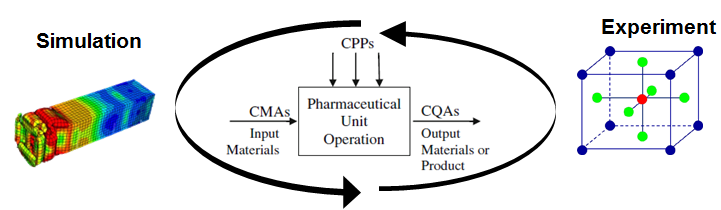
\includegraphics[height=4cm]{img/DesignSpace.PNG}
   \caption{The combination of designed experiments and simulation yields process understanding and finally the design space.}
 \label{fgr:PFS}
\end{figure}
\newpage
\subsection{Research}

\subsubsection{Background}
During the final assembly of pre-filled medical syringes, a polymer rod is snapped into the
rubber stopper, which in turn provides isolation of the liquid medical agent. The resistance
necessary for the snap-in to occur is on the one hand provided by the air pressure compressed between liquid and rubber stopper, and on the other through friction of the stopper with the surrounding glass container. The former is caused by stopper downward movement and it is triggered by a lower break loose force (static friction between the glass barrel internal wall and the stopper) than the pushing plunger rod insertion force. The displacement represents a quality risk to the product as it has the potential to pull contaminants into the drug product but also to further compromise additional component assembly, packaging and finally the patient. The objective is thus to mitigate the risk by minimizing the displacement to assure product conformity to specifications. 
From a computational point of view, this is a challenging problem due to several reasons. Rubber materials mostly obey hyperplastic constitutive relations and thus require FEM formulations able to deal with volumetric locking effects. Furthermore, the snap-in problem itself represents an instability state, which is known to cause convergence issues, which are further deepened by the loosely defined friction conditions.

\subsubsection{Objective}
The primary goal of this thesis is the development of a robust and validated computational
model able to deal with the mentioned challenges and to deliver sufficient accuracy. This will enable the quantification of the plunger stopper displacement for defined process parameters and thus to determine if the product is within the specification or not.
Furthermore, this thesis it is aimed to design a set of real/virtual experiments in order to elucidate the effect of the different factors influencing the process and determine the operating range of the process parameters.

\subsubsection{Methodology}
As mentioned in the background, this work is based on a combination of simulation and experiments. The starting point is the simulation of the assembly process with a representative 2D axisymmetric static model with nominal component specifications. As there are two relative movement phenomena: plunger rod insertion and stopper movement, each are modeled separately at first in order to calibrate the model. In a later stage, the whole process is simulated and then validated with experiments to test the model accuracy. This is then repeated for a dynamic simulation. The second phase involves sensitivity analysis and is performed in order assess the most critical contributing factors to the snap-in. Designed experiments also serve as validation tool for selected factors.

\newpage
\subsection{Outline}
The thesis is organized as follows. First, an introduction is given in the 1st chapter with the motivations, objectives and context of this work. Then, relevant literature is presented and analyzed in the 2nd chapter first in the context of pre-filled syringes and secondly, for finite element related problems with emphasis on hyperelastic, contact and instability modeling.
Afterwards the theoretical framework of process modelling in chapter 3 and then of finite element modeling is exposed. Specifically, the basics of nonlinear, hyperelastic, contact modeling are explained in the chapters 4, 5 and 6. 
The 7th chapter illustrates  the input data used for ANSYS is including the material data generation and the CAD geometry. 
Then, some initial considerations are given regarding the physics and the important parameters of the assembly process in chapter 8. Afterwards, the results of the FE analysis  for both the static and dynamic cases are exposed and discussed in conjunction with the validation experiments in chapter 9. A critical inflection is given on the validity on the model and put in context with the results of sensitivity analysis. Chapter 10 illustrates the obtained experimental results from the experimental design and statistical results.
Finally, the conclusion and an outlook are given in chapter 11.

